%% GENERATED by tools/from_docs.py from stepss-docs. Do not edit by hand:
%% edit the page named below in stepss-docs and regenerate.
%% source: stepss-docs/src/content/docs/models/discrete-controllers/tap-changers.md

\chapter{Tap changer controllers}\label{doc:model-dctl-ltc}

The \texttt{DCTL} record these models are entered with, and the rules on model names, are on the \hyperref[doc:model-dctl]{Discrete Controller Models} page.

\begin{docsnote}{TRFO and DCTL LTC}

The \hyperref[ch-network]{TRFO record} combines the transformer model with load tap changer data (tap range, positions, controlled bus, voltage setpoint), but this data is used \textbf{only by the power flow} for ratio adjustment. To control a transformer's ratio during dynamic simulation with RAMSES, a DCTL LTC controller (below) must be associated with the transformer, whether it was defined with TRANSFO or TRFO.

\end{docsnote}

Every controller in this section is a timed automaton rather than a transfer
function: it watches a quantity, waits out a delay, then acts. The tap changers
share the sequence below, and differ only in how the delay is computed.

\begin{figure}[htbp]
\centering
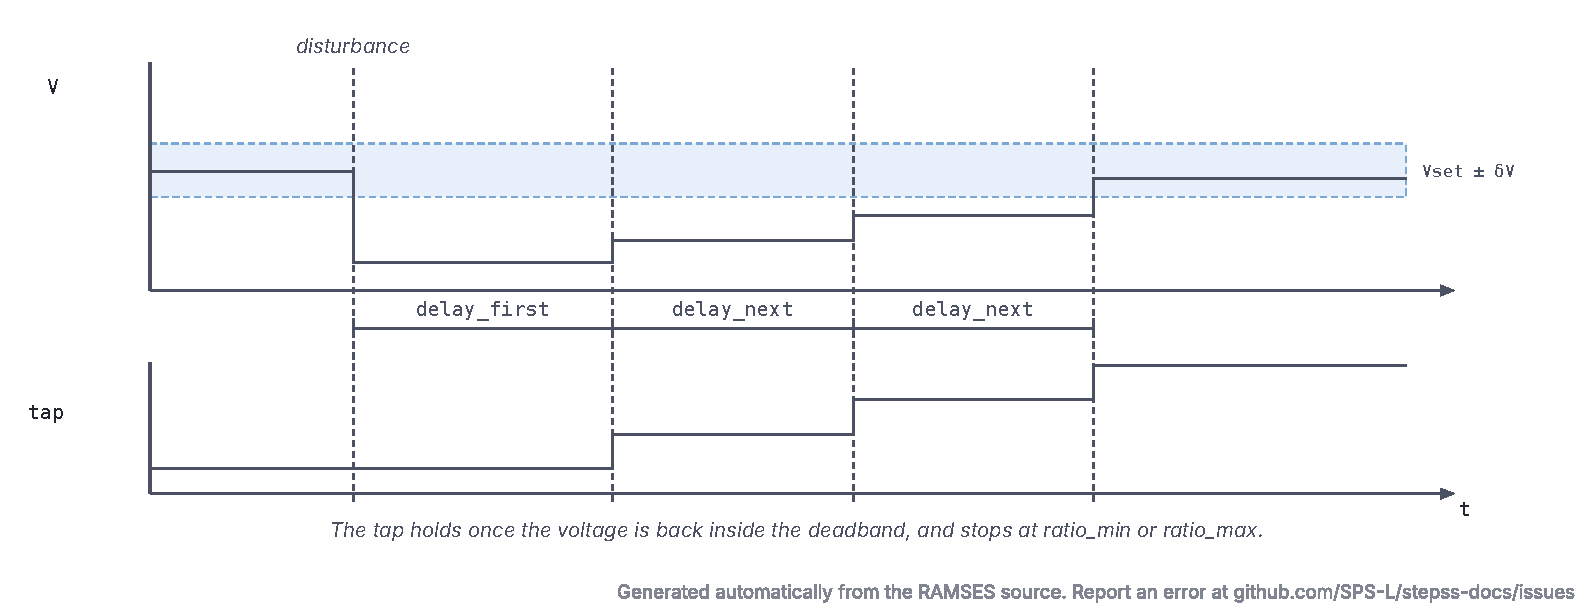
\includegraphics[width=0.98\linewidth]{figures/dctl-ltc-timing-light}
\caption{Tap changer timing diagram.}
\end{figure}

\section{\texorpdfstring{LTC (\texttt{dctl\_ltc}): Load Tap Changer (Standard)}{LTC (dctl\_ltc): Load Tap Changer (Standard)}}\label{model-dctl-ltc:ltc-dctl_ltc-load-tap-changer-standard}

\subsection{Description}\label{model-dctl-ltc:description}

Controls the ratio of a transformer to regulate voltage at a \textbf{monitored bus}. It monitors the voltage, compares it against a deadband around the setpoint (initialised to the voltage at \(t=0\)), and initiates a tap change after a delay if the voltage remains outside the deadband.

The first tap change uses a longer delay (\texttt{delay\_first}); subsequent changes use a shorter delay (\texttt{delay\_next}), implementing the standard IEC/IEEE slow-start behaviour.

\subsection{Logic Description}\label{model-dctl-ltc:logic-description}

Let \(V\) be the monitored bus voltage and \(V_{set}\) the setpoint:

\[\text{Error} = V_{set} - V\]

\textbf{Deadband check}: No action if \(|V - V_{set}| \le \delta V\) (half-deadband).

\textbf{Direction logic}: If \texttt{direction\ \textgreater{}\ 0}, increasing the ratio increases the voltage.

\textbf{Timer logic}:

\[\text{if } |V - V_{set}| > \delta V \text{ and } (t - t_{last}) \ge \tau_{delay}:
\quad \text{tap} \leftarrow \text{tap} \pm \Delta r, \quad t_{last} \leftarrow t\]

where \(\tau_{delay} = \tau_{first}\) for the first operation, \(\tau_{next}\) thereafter, and the tap is clamped to \([r_{\min}, r_{\max}]\).

\textbf{State variable} \texttt{w(13)}:
- \texttt{0}: voltage within deadband
- \texttt{+1}: \(V < V_{set} - \delta V\) (tap must increase)
- \texttt{\ensuremath{-}1}: \(V > V_{set} + \delta V\) (tap must decrease)

\subsection{Parameters}\label{model-dctl-ltc:parameters}

\begin{small}\begin{longtable}[]{@{}
  >{\raggedright\arraybackslash}p{(\linewidth - 6\tabcolsep) * \real{0.2626}}
  >{\raggedright\arraybackslash}p{(\linewidth - 6\tabcolsep) * \real{0.1923}}
  >{\raggedright\arraybackslash}p{(\linewidth - 6\tabcolsep) * \real{0.5451}}
@{}}
\toprule\noalign{}
\begin{minipage}[b]{\linewidth}\raggedright
Field
\end{minipage} & \begin{minipage}[b]{\linewidth}\raggedright
Working variable
\end{minipage} & \begin{minipage}[b]{\linewidth}\raggedright
Description
\end{minipage} \\
\midrule\noalign{}
\endhead
\bottomrule\noalign{}
\endlastfoot
\texttt{branch\_name} & \texttt{w(1)} & Transformer branch name (must be type \texttt{trfo}) \\
\texttt{bus\_name} & \texttt{w(2)} & Monitored (controlled) bus name \\
\texttt{direction} & \texttt{w(3)} & Sign convention: \textgreater0 means increasing ratio raises voltage \\
\texttt{ratio\_min} & \texttt{w(4)} & Minimum transformer ratio (\textbf{\% of nominal}, e.g.~\texttt{85.} for 0.85 pu) \\
\texttt{ratio\_max} & \texttt{w(5)} & Maximum transformer ratio (\textbf{\% of nominal}, e.g.~\texttt{115.} for 1.15 pu) \\
\texttt{nb\_positions} & \texttt{w(6)} & Number of tap positions (step = (max\ensuremath{-}min)/(nb\ensuremath{-}1)) \\
\texttt{half\_deadband} & \texttt{w(7)} & Voltage half-deadband \(\delta V\) (pu) \\
\texttt{delay\_first} & \texttt{w(8)} & Delay before first tap change (s) \\
\texttt{delay\_next} & \texttt{w(9)} & Delay between subsequent tap changes (s) \\
\end{longtable}\end{small}

\begin{docsnote}{Caution}

The ratio limits are given in \textbf{percent}, not per unit: the model divides \texttt{ratio\_min} and \texttt{ratio\_max} by 100 when reading the data. A record with \texttt{0.85\ 1.15} would silently produce limits of 0.0085/0.0115 pu.

\end{docsnote}

\subsection{Usage Example}\label{model-dctl-ltc:usage-example}

\begin{Verbatim}
DCTL  LTC  LTC_TR1
      # branch: transformer whose ratio is controlled
      TR1-HV-MV
      # bus: bus whose voltage is controlled
      BUS_MV
      # direction: sign of the ratio change that raises the voltage (only the sign is used, 0 is refused)
      1
      # ratio_min: minimum ratio (%)
      85.
      # ratio_max: maximum ratio (%)
      115.
      # nb_positions: number of tap positions, at least 2
      33
      # half_deadband: half of the voltage deadband (pu)
      0.01
      # delay_first: delay before the first tap change (s)
      30.0
      # delay_next: delay between subsequent tap changes (s)
      10.0
;
\end{Verbatim}

\begin{center}\rule{0.5\linewidth}{0.5pt}\end{center}

\section{\texorpdfstring{LTC2 (\texttt{dctl\_ltc2}): Load Tap Changer (Variant 2)}{LTC2 (dctl\_ltc2): Load Tap Changer (Variant 2)}}\label{model-dctl-ltc:ltc2-dctl_ltc2-load-tap-changer-variant-2}

\subsection{Description}\label{model-dctl-ltc:description-1}

Identical logic to \texttt{dctl\_ltc} but the \textbf{voltage setpoint is an explicit input parameter} rather than being taken from the initial operating point. This allows prescribing a setpoint different from the initial bus voltage, which is useful when the initial load-flow voltage differs from the desired operating voltage.

\subsection{Logic Description}\label{model-dctl-ltc:logic-description-1}

Same deadband, direction, and timer logic as \texttt{dctl\_ltc}. The voltage setpoint \(V_{set}\) is read directly from the data field \texttt{Vset} instead of being captured at \(t = 0\).

\[\text{if } |V - V_{set}| > \delta V \text{ and } (t - t_{last}) \ge \tau_{delay}: \quad \text{tap change}\]

\subsection{Parameters}\label{model-dctl-ltc:parameters-1}

\begin{small}\begin{longtable}[]{@{}lll@{}}
\toprule\noalign{}
Field & Working variable & Description \\
\midrule\noalign{}
\endhead
\bottomrule\noalign{}
\endlastfoot
\texttt{branch\_name} & \texttt{w(1)} & Transformer branch (type \texttt{trfo}) \\
\texttt{bus\_name} & \texttt{w(2)} & Monitored bus \\
\texttt{direction} & \texttt{w(3)} & \textgreater0: ratio increase raises voltage \\
\texttt{ratio\_min} & \texttt{w(4)} & Minimum ratio (\% of nominal) \\
\texttt{ratio\_max} & \texttt{w(5)} & Maximum ratio (\% of nominal) \\
\texttt{nb\_positions} & \texttt{w(6)} & Number of tap positions \\
\texttt{half\_deadband} & \texttt{w(7)} & Voltage half-deadband (pu) \\
\texttt{Vset} & \texttt{w(8)} & Voltage setpoint (pu) \\
\texttt{delay\_first} & \texttt{w(9)} & First tap change delay (s) \\
\texttt{delay\_next} & \texttt{w(10)} & Subsequent tap change delay (s) \\
\end{longtable}\end{small}

\subsection{Usage Example}\label{model-dctl-ltc:usage-example-1}

\begin{Verbatim}
DCTL  LTC2  LTC2_TR1
      # branch: transformer whose ratio is controlled
      TR1-HV-MV
      # bus: bus whose voltage is controlled
      BUS_MV
      # direction: sign of the ratio change that raises the voltage (only the sign is used, 0 is refused)
      -1
      # ratio_min: minimum ratio (%)
      88.
      # ratio_max: maximum ratio (%)
      120.
      # nb_positions: number of tap positions, at least 2
      33
      # half_deadband: half of the voltage deadband (pu)
      0.01
      # Vset: voltage setpoint (pu)
      1.0
      # delay_first: delay before the first tap change (s)
      30
      # delay_next: delay between subsequent tap changes (s)
      8
;
\end{Verbatim}

\begin{center}\rule{0.5\linewidth}{0.5pt}\end{center}

\section{\texorpdfstring{LTCINV (\texttt{dctl\_ltcinv}): Inverse-Time Load Tap Changer}{LTCINV (dctl\_ltcinv): Inverse-Time Load Tap Changer}}\label{model-dctl-ltc:ltcinv-dctl_ltcinv-inverse-time-load-tap-changer}

\subsection{Description}\label{model-dctl-ltc:description-2}

An \textbf{inverse-time} tap changer in which the delay before a tap change is proportional to the integral of the voltage deviation rather than a fixed timer. Large voltage errors trigger faster operation; small but persistent deviations trigger slower operation.

This implements behaviour analogous to inverse-time overcurrent relays, applied to voltage control.

\subsection{Logic Description}\label{model-dctl-ltc:logic-description-2}

The controller integrates the signed voltage deviation over time:

\[\Sigma = \int_{t_0}^{t} (V_{set} - V) \, dt'\]

A tap change fires when the integrated error exceeds a threshold derived from the maximum delay and acceleration parameter:

\[\text{if } |\Sigma| \ge \frac{\tau_{max} \cdot \delta V}{\text{accel}}: \quad \text{tap change}, \quad \Sigma \leftarrow 0\]

where \(\tau_{max}\) is the maximum delay and \texttt{accel} is the acceleration factor (smaller value = faster response).

\textbf{State variable} \texttt{w(13)}: same coding as \texttt{dctl\_ltc}.

\subsection{Parameters}\label{model-dctl-ltc:parameters-2}

\begin{small}\begin{longtable}[]{@{}lll@{}}
\toprule\noalign{}
Field & Working variable & Description \\
\midrule\noalign{}
\endhead
\bottomrule\noalign{}
\endlastfoot
\texttt{branch\_name} & \texttt{w(1)} & Transformer branch \\
\texttt{bus\_name} & \texttt{w(2)} & Monitored bus \\
\texttt{direction} & \texttt{w(3)} & Sign convention \\
\texttt{ratio\_min} & \texttt{w(4)} & Minimum ratio (\% of nominal) \\
\texttt{ratio\_max} & \texttt{w(5)} & Maximum ratio (\% of nominal) \\
\texttt{nb\_positions} & \texttt{w(6)} & Number of tap positions \\
\texttt{half\_deadband} & \texttt{w(7)} & Voltage half-deadband (pu) \\
\texttt{Vset} & \texttt{w(8)} & Voltage setpoint (pu) \\
\texttt{delay\_max} & \texttt{w(9)} & Maximum delay before tap change (s) \\
\texttt{accel} & \texttt{w(10)} & Acceleration factor (s), smaller = faster \\
\end{longtable}\end{small}

\subsection{Usage Example}\label{model-dctl-ltc:usage-example-2}

\begin{Verbatim}
DCTL  LTCINV  LTCINV_TR1
      # branch: transformer whose ratio is controlled
      TR1-HV-MV
      # bus: bus whose voltage is controlled
      BUS_MV
      # direction: sign of the ratio change that raises the voltage (only the sign is used, 0 is refused)
      1
      # ratio_min: minimum ratio (%)
      85.
      # ratio_max: maximum ratio (%)
      115.
      # nb_positions: number of tap positions, at least 2
      33
      # half_deadband: half of the voltage deadband (pu)
      0.01
      # Vset: voltage setpoint (pu)
      1.025
      # delay_max: delay for a voltage error equal to the half deadband (s)
      60.0
      # accel: time subtracted from the inverse-time delay (s)
      0.1
;
\end{Verbatim}

\begin{center}\rule{0.5\linewidth}{0.5pt}\end{center}

\section{\texorpdfstring{OLTC2 (\texttt{dctl\_oltc2}): On-Load Tap Changer Type 2}{OLTC2 (dctl\_oltc2): On-Load Tap Changer Type 2}}\label{model-dctl-ltc:oltc2-dctl_oltc2-on-load-tap-changer-type-2}

\subsection{Description}\label{model-dctl-ltc:description-3}

An advanced on-load tap changer with \textbf{R/X line drop compensation}, end-stop flags. It includes separate flags to prevent tap movement when the transformer is at its mechanical end-stop, and applies voltage correction based on the current flowing through the transformer using the compensation resistances \texttt{R\_comp} and \texttt{X\_comp}.

The \textbf{Ratio2-factor} enables a secondary correction factor for the transformer ratio independent of the main tap position.

\subsection{Logic Description}\label{model-dctl-ltc:logic-description-3}

Compensated voltage seen by the controller:

\[V_{comp} = V_{meas} - R_{comp} \, I_{re} - X_{comp} \, I_{im}\]

where \(I_{re}, I_{im}\) are the real and imaginary components of the transformer current. The deadband check and timer logic then operate on \(V_{comp}\).

End-stop flags \texttt{w(15)} and \texttt{w(16)} prevent further tap changes when the ratio is already at its limit and the requested change would move it beyond.

\subsection{Parameters}\label{model-dctl-ltc:parameters-3}

\begin{small}\begin{longtable}[]{@{}lll@{}}
\toprule\noalign{}
Field & Working variable & Description \\
\midrule\noalign{}
\endhead
\bottomrule\noalign{}
\endlastfoot
\texttt{branch\_name} & \texttt{w(1)} & Transformer branch \\
\texttt{bus\_name} & \texttt{w(2)} & Controlled bus \\
\texttt{direction} & \texttt{w(3)} & Sign convention \\
\texttt{ratio\_min} & \texttt{w(4)} & Minimum ratio (pu) \\
\texttt{ratio\_max} & \texttt{w(5)} & Maximum ratio (pu) \\
\texttt{nb\_positions} & \texttt{w(6)} & Number of tap positions \\
\texttt{half\_deadband} & \texttt{w(7)} & Voltage half-deadband (pu) \\
\texttt{Vset} & \texttt{w(8)} & Voltage setpoint (pu) \\
\texttt{delay\_first} & \texttt{w(9)} & First tap change delay (s) \\
\texttt{delay\_next} & \texttt{w(10)} & Subsequent tap change delay (s) \\
\texttt{R\_comp} & \texttt{w(17)} & Line drop compensation resistance (pu) \\
\texttt{X\_comp} & \texttt{w(18)} & Line drop compensation reactance (pu) \\
\texttt{ratio2\_factor} & \texttt{w(20)} & Secondary ratio correction factor (pu) \\
\end{longtable}\end{small}

14 fields required (includes from-bus, to-bus, circuit ID for PSS/E format).

\subsection{Usage Example}\label{model-dctl-ltc:usage-example-3}

\begin{Verbatim}
DCTL  OLTC2  OLTC_TR2
      # branch: transformer whose ratio is controlled
      TR1-HV-MV
      # bus: bus whose voltage is controlled
      BUS_MV
      # direction: sign of the ratio change that raises the voltage (0 locks the tap)
      1
      # ratio_min: minimum ratio (%)
      88.
      # ratio_max: maximum ratio (%)
      112.
      # nb_positions: number of tap positions, at least 2
      25
      # half_deadband: half of the voltage deadband (pu)
      0.0075
      # Vset: voltage setpoint; the initial voltage must lie within Vset +/- half_deadband (pu)
      1.02
      # delay_first: delay before the first tap change (s)
      45.0
      # delay_next: delay between subsequent tap changes (s)
      15.0
      # R_comp: line-drop compensation resistance (pu)
      0.0
      # X_comp: line-drop compensation reactance (pu)
      0.0
      # verbose: 1 = full log messages; any other value gives fewer
      1
      # ratio2_factor: scales the tap ratio printed in log messages only
      1.0
;
\end{Verbatim}
